%%%%%%%%%%%%%%%%%%%%%%%%%%%%%%%%%%
% Chapter 1 
%%%%%%%%%%%%%%%%%%%%%%%%%%%%%%%%%%
\chapter{INTRODUCTION}
%%
%%
%%      1
%%
%%
\section{Reproducibility}
The trustworthiness of scientific research is maintained through the
processes of peer review and study reproduction. In the former, expert readers
screen work submitted for publication, providing commentary and recommendations
on the work’s validity and publication merit. In the latter, scientific
questions are revisited, often by new researchers, in efforts to support or
disprove original results.

As defined in a report by the U.S. National Science foundation,
“reproducibility refers to the ability of a researcher to duplicate the results
of a prior study using the same materials as were used by the original
investigator. That is, a second researcher might use the same raw data to build
the same analysis files and implement the same statistical analysis in an
attempt to yield the same results…. Reproducibility is a minimum necessary
condition for a finding to be believable and informative” \parencite[3]{cacioppo_social_2015}.

The documentation of research with reproducibility in mind is critical to
both the peer review process and the process of study reproduction itself. A
reviewer may not have the confidence to recommend the publication of submitted
work if efforts have not been made to ensure its reproducibility, and without
the building blocks of reproducibility, researchers are unlikely to be able to
support study findings through further work. Furthermore, inadequately
documented research may reduce the potential value of a study to the scientific
community, by preventing inference about methods or results, expansion, or
extension towards more general findings.

Defining core concepts in reproducibility has been the subject of
significant recent work, and is beyond our scope here. \textcite{plesser_reproducibility_2018}
provides a useful overview of common terminology schemes, including the
following simplification of Goodman’s terminology \parencite{goodman_what_2016},
which we will adopt for the remainder:
\begin{quote}
    \begin{itemize}
        \item Methods reproducibility: provide sufficient detail about procedures and data so that the same procedures [can] be exactly repeated.
        \item Results reproducibility: obtain the same results from an independent study with procedures as closely matched to the original study as possible.
        \item Inferential reproducibility: draw the same conclusions from either an independent replication of a study or a reanalysis of the original study. (3)
    \end{itemize}
\end{quote}
Goodman is broadly concerned with the “operationalization of truth” in science,
and these three types of reproducibility support the truthfulness of a study in
specific ways. A study that achieves methods reproducibility can be directly
corroborated through repetition or replication. Results reproducibility is
achieved through the independent enactment of this corroborating work, and so
supports the idea that the original study results were valid. Inferential
reproducibility, a broader and potentially more meaningful goal, takes the final
step of supporting the validity of the conclusions drawn in the original work
with the results of a reproduction study.

There has been much recent discussion in the scientific community about a
contemporary “reproducibility crisis”, and it is important that we draw a
distinction between two different types of reproducibility failure. High-profile
publications on the topic (\cite{open_science_collaboration_estimating_2015}; \cite{baker_1500_2016})
are concerned primarily with failures of results reproducibility or inferential
reproducibility: researchers are unable to corroborate the findings of the
original published work, but may be able to reproduce the methods used. This
does not lessen the importance of these findings. Failure to corroborate large
swaths of published work has the potential to undermine public trust in science,
and it is a testament to the scientific method that this kind of critical work
is being done.

These publications may underplay the lower-level issue that many studies
fail to achieve even the level of documentation required for methods
reproducibility. As Goodman writes, “the modern use of ‘reproducible research’
was originally applied not to corroboration, but to transparency, with
application in the computational sciences. Computer scientist Jon Claerbout
coined the term and associated it with a software platform and set of procedures
that permit the reader of a paper to see the entire processing trail from the
raw data and code to figures and tables”\parencite[1]{goodman_what_2016}.
\textcite{stark_before_2018} proposes a new term,
“preproducibility”, targeting this distinction between studies that are
adequately documented for reproduction and those which are not. In this
model, a “preproducible” study is one whose methods have been adequately
documented, and preproducibility is a precondition for reproducibility. In this
thesis, we are primarily concerned with this fundamental problem - failures in
methods reproducibility preclude any effort at higher levels of corroboration,
and failures in documentation may preclude methods reproducibility.

%%
%%
%%    2
%%   
%%
\section{Provenance}

All three of the types of reproducibility discussed above share methods
reproducibility as a base requirement, and all require the same high level of
effort to enact in practice, or, to use Goodman’s term, to operationalize. In
the field of computational biology, and less broadly, in microbiome
bioinformatics, researchers frequently work with large and expensive data sets,
advanced computer hardware, complex software systems, large numbers of
variables, and analytical processes with tens or even hundreds of steps. In
order to achieve methods reproducibility in studies like these, a researcher
must have access to:
\begin{itemize}
    \item original or similar raw data
    \item original or similar study metadata
    \item computational resources including the same software and software versions originally used
    \item comprehensive reporting of the analytical process, including analysis steps and all relevant parameter settings - in other words, what the user did with the data and metadata on the system.
\end{itemize}
This is a high bar to clear, and researchers may not be incentivized to
adequately invest resources into achieving it. Others have the best intentions,
but do not know what information needs to be documented, or how to do so
appropriately (e.g. capturing details of the computing environment, using
resource identification schemes that are resilient to filename changes).
Contemporary researchers must manage a high volume of new information and many
competing requirements for their time, while publication, promotion and funding
structures tend to prioritize high-impact new work over reproduction
(\cite{community_turing_2021}; \cite{shiffrin_scientific_2018}; \cite{munafo_manifesto_2017}).
There is an inherent tension between the idea that reproducibility is a
pre-condition for trust, and the fact that studies may not be funded to cover
the overhead costs associated with reproducibility.

At a minimum, a reproducible research outcome must document the systems and
processes upon which it depends. Put differently, published results must include
information about their own derivation history, or provenance, which others can
use in reproducing their analytical systems and methods. The nomenclature of
provenance data capture provides useful context. According to Zhao et al,
approaches to provenance tracking can be broken down into "the aspects of the
procedure or workflow used to create a data object (prospective provenance, or
“recipe”)... [and] information about the runtime environment in which a
procedure was executed and the resources used in its invocation (retrospective
provenance)" \parencite[149]{hutchison_applying_2006}. There are many different ways
to serve one or both of these needs. Prospective approaches may include tools
for the annotation of executable code and/or the generation of documentation
from executable code (e.g. Jupyter Notebooks, RMarkdown), or may be based on
workflow automation specifications with tools like Common Workflow Language
(CWL) or NextFlow. The paradigm here is frequently one in which a provenance
document is written by the user and then executed to produce the results.
Retrospective approaches function by capturing information about an analysis
during execution. Benefits to this approach include the ability to record
information about the underlying system at run time, including hardware and
software environments, resource use, passed data and metadata, and identifiers
for both intermediate and final results. Hybrid approaches have also been
developed, blending prospective and retrospective methods \parencite{zhang_revealing_2017}.

%%
%%
%%    3
%%   
%%
\section{Provenance in QIIME 2}

This work targets the QIIME 2 platform for microbiome bioinformatics, which
uses a decentralized, retrospective approach to provenance tracking. QIIME 2 is,
conceptually, an application framework designed to expose plugin-defined
bioinformatics methods for use via a variety of (potentially user-defined) user
interfaces. In addition to facilitating this behavior, the framework implements
functionality required universally, including systems for recording QIIME 2
results and for capturing provenance data. “Details of all analysis steps with
references to intermediate data are automatically stored in the results. Users
can thus retrospectively determine exactly how any result was generated \parencite[854]{bolyen_reproducible_2019}”.
Key to understanding this model is the idea that provenance capture is
decentralized, with provenance data stored in results, rather than storing it in
some centralized resource or relying on users to correctly associate research
outputs with the code that generated them. Every visualization or data output
created by QIIME 2 contains a full history of the analysis that produced it.
(See figure \ref{fig:provenance_graph})

\begin{figure}[htp]
\centering
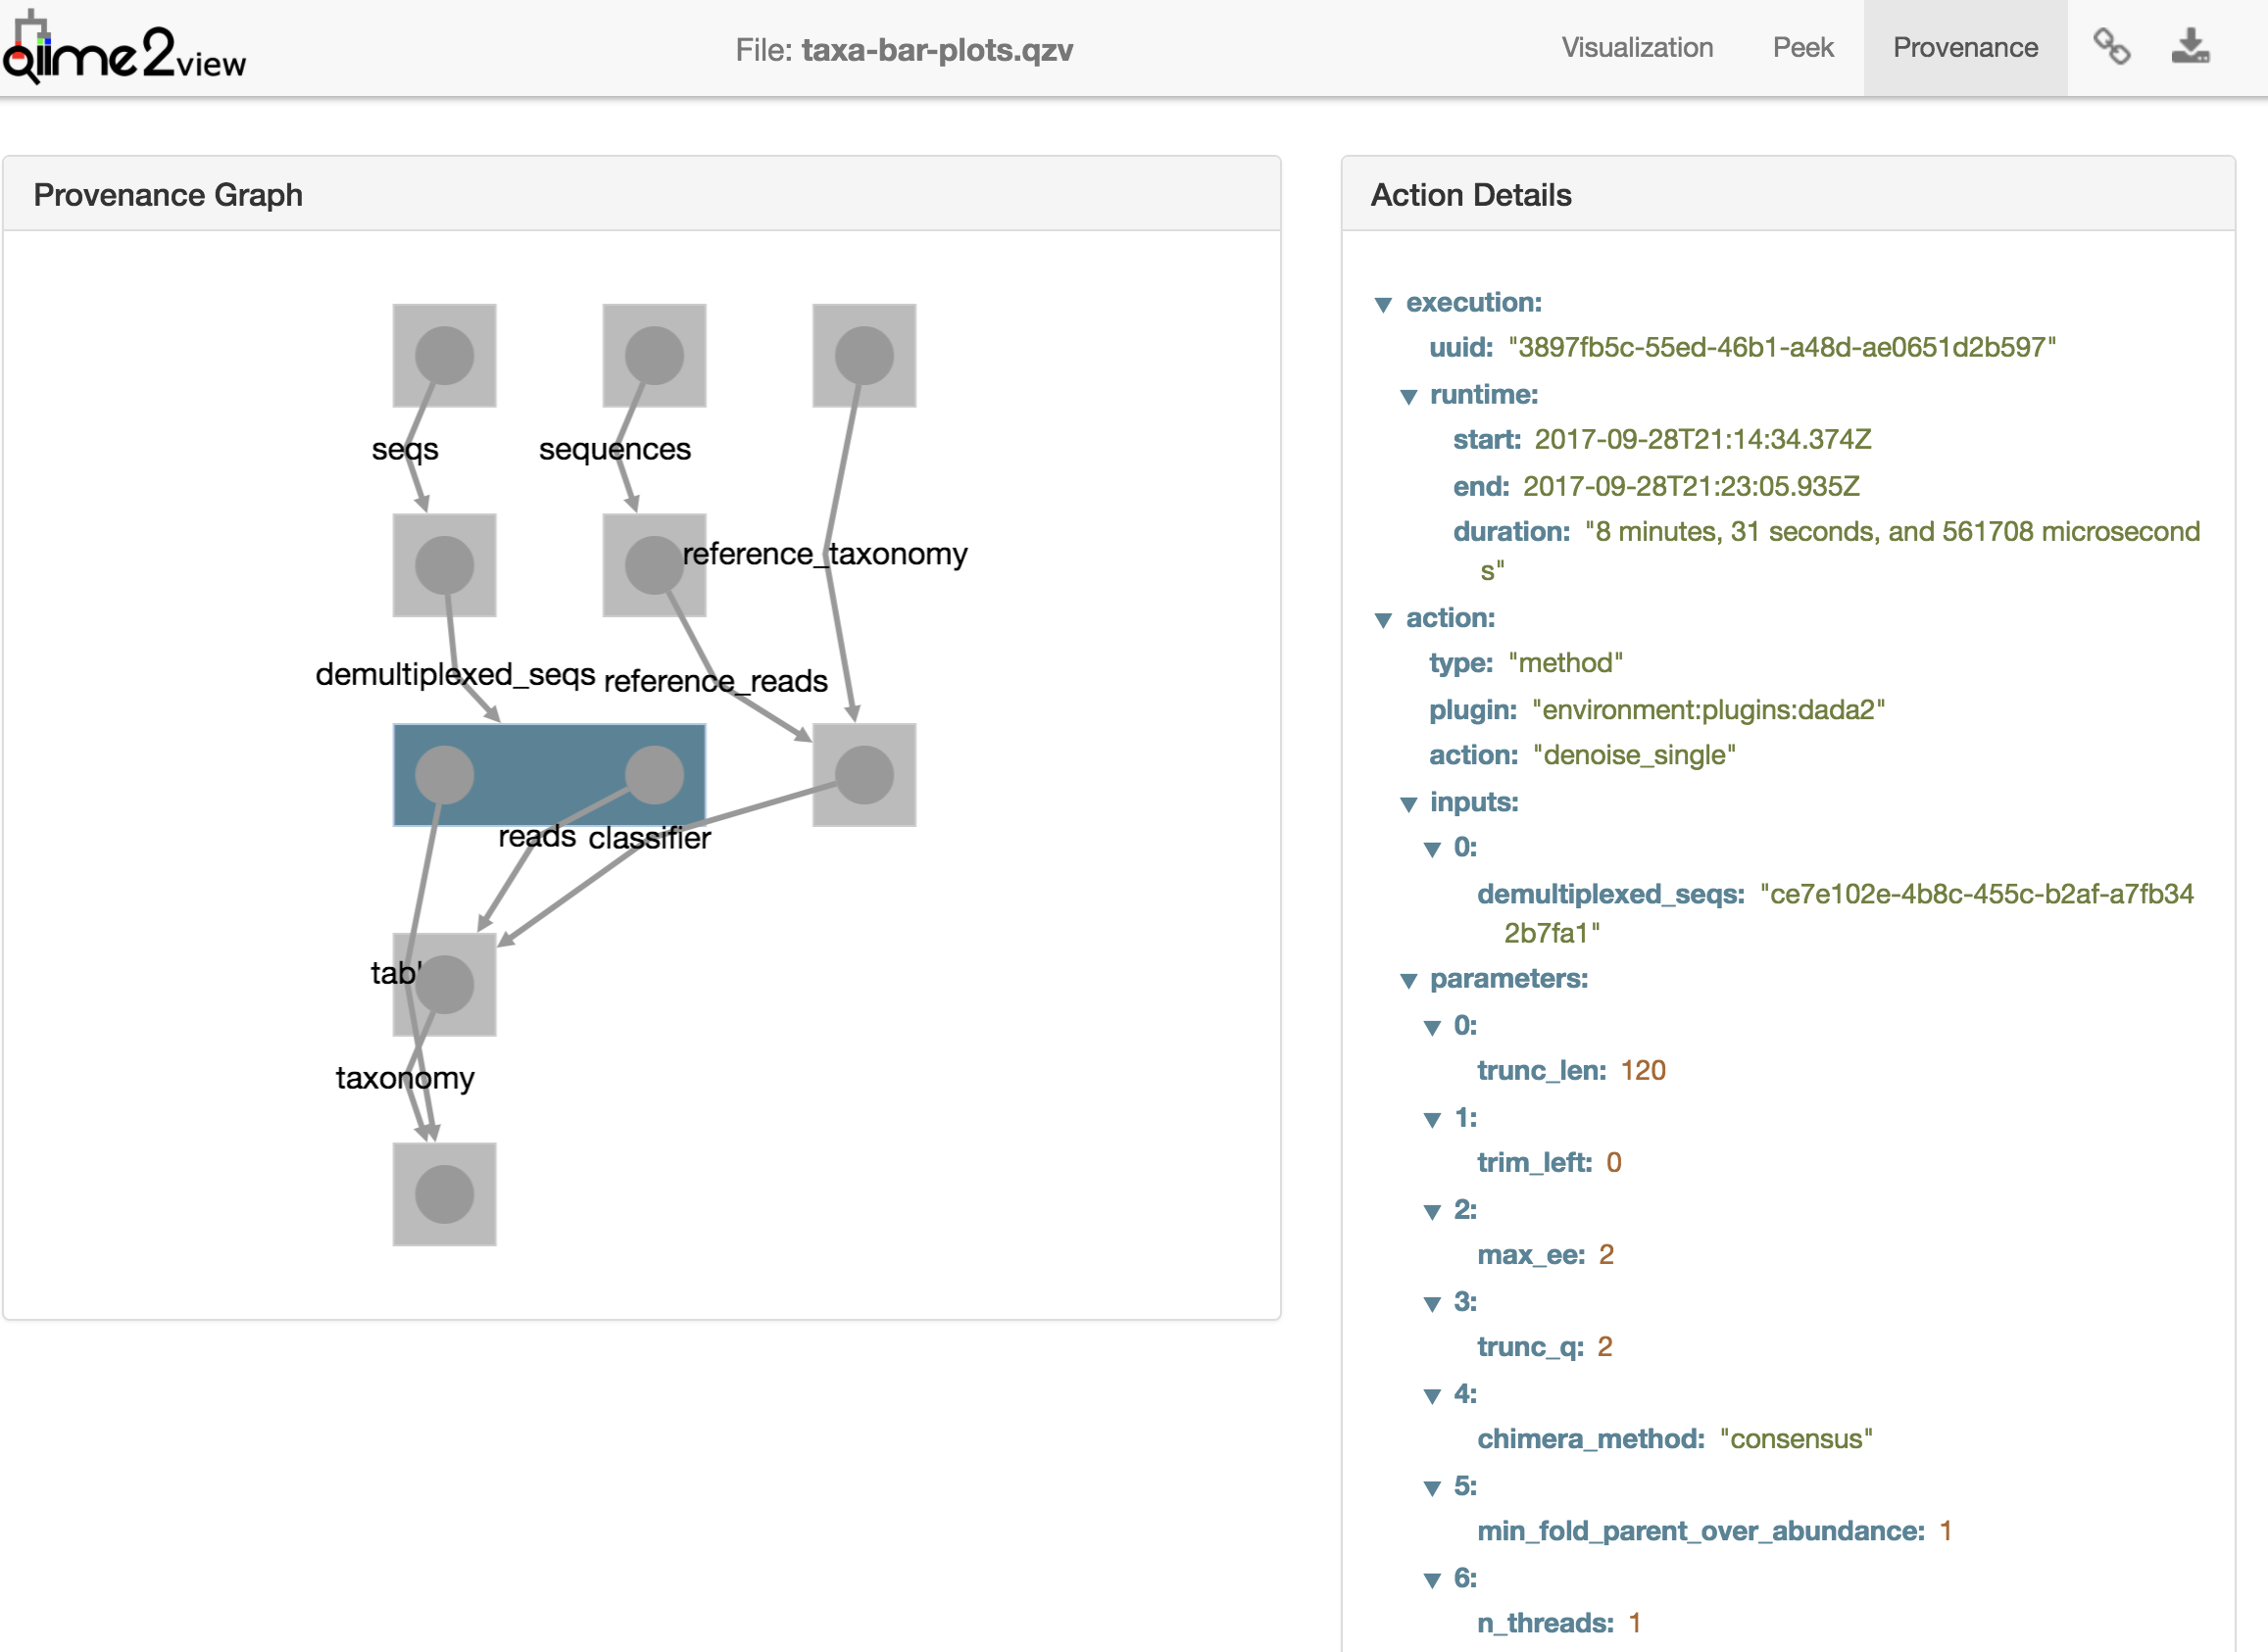
\includegraphics[width=\textwidth]{figures/provenance_graph.png}
\caption[Diagram of the history (provenance) of a QIIME 2 Artifact]%
{Diagram of the history (i.e. provenance) of a QIIME 2 Artifact. At left, a
directed, acyclic graph tracing this history from initial data import into QIIME
2, through the creation of a visualization for analytical interpretation or
publication, from top to bottom. Graph nodes represent QIIME 2 results, and
edges represent the actions performed to produce them. Graph nodes are composed
of one or more circles inside of a rectangle. The circles represent Results, and
the rectangles represent the actions that produced those results. (An Action may
produce one or more Results.) Graph edges describe the “movement” of Results
through an analysis; an edge originates in some Result, and “points at” any
Actions that used that result as an input. At right are the “action details”
captured during the creation of the two nodes highlighted in blue. QIIME 2
captures unique result identifiers, software version information, details on all
commands and parameters used, and computational resource use.}
\label{fig:provenance_graph}
\end{figure}

\textcite{khan_sharing_2019} propose a framework of best practices for provenance capture,
many of which are satisfied by QIIME 2’s existing provenance capture system.
Data processing is done with versioned software rather than manual data
manipulation. All commands executed are recorded, along with their parameters,
and the versions of software they ran on. These software environments are
documented in provenance at run time, using the git version control system to
indicate modifications made to installed QIIME 2 packages. Basic information on
the hardware environment is recorded. Human-interpretable diagrams of result
history can be easily generated from any result and explored in a web browser
with no software installation needed. Result “archives” are formatted
consistently in clearly-defined ways, and when stored on disk they are packaged
in a common zip file format that is likely to be accessible across systems for
the foreseeable future.

The primary theoretical requirements for reproducing an in silico analysis in
QIIME 2 are met. However, the practical costs of doing so remain prohibitive.
Consider a relatively straightforward QIIME 2 analysis of a longitudinal data
set. We might import data from a single run of biological sequences generated by
a sequencing machine, and then analyze it, visualizing taxonomic composition,
alpha and beta diversity, changes in some important metrics over time, and
differential abundance between samples of interest. This analysis might require
25-30 discrete commands be run, producing 100 data outputs and figures. In order
to reproduce the analysis manually, the user would need to assemble each of
those commands from the serialized “action detail” data captured in provenance. 

In addition, the decentralized nature of QIIME 2’s provenance capture means that
history is captured on a per-result basis. There is no representation of a
complete workflow or analysis. In order to recreate a workflow, then, the user
must “re-assemble” a meaningful analysis from the provenance of many different
QIIME 2 results. This would require a clear understanding of what all of those
results are and what they mean in the context of the analysis, or a tremendous
and often redundant effort, reading the provenance of all 100 result objects and
knitting them together into runnable code for the 25-30 actions that produced
them. Even if we could assume user expertise sufficient to do the work
efficiently, the process would be painstaking and prone to human error. 

%%
%%
%%      4
%%
%%
\section{Reproducible research goals}
\label{section:repro_goals}

Breaking the expertise barrier described above has been a target of
computational reproducibility since at least Claerbout in 1992, whose team
published scientific work in digital media, and included in each figure’s
caption references and/or buttons that allowed trivial re-running of the
analysis that created that figure. They claimed that in this reproducible work,
“[j]udgement of the reproducibility of computationally oriented research no
longer requires an expert—a clerk can do it” (as cited in \cite[76]{plesser_reproducibility_2018}).
This “one-click” approach to reproducibility provides clear value for its
simplicity in corroborating the provenance of a single figure, and so is a
useful end goal to consider in the broader context of possible positive outcomes
from reproducible research.

Gunderson and Kjensmo, in their work on reproducibility in Artificial
Intelligence (AI), propose a hierarchical three-value system for ranking the
reproducibility of an AI based upon that AI’s degree of generality:
\begin{itemize}
    \item Experiment Reproducible systems “produce the same results when [the same implementation is] executed on the same data."
    \item Data Reproducible systems produce the same results when executing “an alternative implementation of the AI method… on the same data.”
    \item Method Reproducible systems produce the same results when executing “an alternative implementation of the AI method… on different data” \parencite[4]{gundersen_state_2018}.
\end{itemize}
% TODO: Inexplicably, the rest of the document indents if we don't end twice here.
\end{itemize}

\noindent The Turing Way Community’s definitions of “Reproducible”, “Robust”, and
“Generalisable” align (respectively) with these definitions, but exchange a
clear ordering for the ability to include an additional combination of factors,
defining:

\begin{itemize}
    \item “Replicable” systems “produce qualitatively similar answers”, when “the same analysis is performed on different datasets” \parencite{community_definitions_2021}.
\end{itemize}

\noindent Though varying slightly in scope and intent, these two systems both classify
distinct “types of reproducibility”, based on study design or outcome. There is
no “correct” or standard nomenclature in the literature, so we will impose a
Gunderson-like hierarchy on the Turing Way terminology here. (Figure \ref{fig:repro_classes})

\begin{figure}[htbp]
\centering
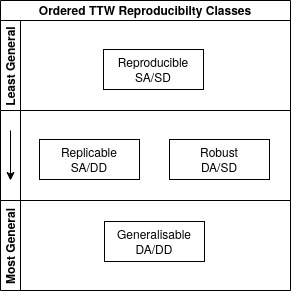
\includegraphics[width=.5\textwidth]{figures/repro_outcomes.jpg}
\caption[Hierarchically arranged reproducibility classes]%
{In this figure, Turing Way reproducibility classes are ordered in a
Gunderson-like hierarchy based on generality. Each class includes a pair of
descriptive two-letter codes, where the first letter abbreviates either Same or
Different, and the second letter Data or Analysis. For example, a Robust study
is coded DA/SD because it achieves the same results using a Different Analysis
of the Same Data.}
\label{fig:repro_classes}
\end{figure}

The value of Claerbout’s simple “one-click” approach breaks down once we
acknowledge that the fundamental goals of reproducibility often extend beyond
simple corroboration. As Shiffrin et al put it, "an effect valid in only one
exact context and not others is not usually useful and important. We want to
report effects that are reliable, important, are of scientific value, and
generalize to similar settings" \parencite[2633]{shiffrin_scientific_2018}.
A one-click-reproducible figure achieves only “reproducibility” - the lowest
level of generality. It allows us to corroborate that the software and the data
produce a deterministic result, but tells us nothing meaningful about the
correctness of either. Investigating this further would still require an expert
to consider the data, read the source code, and make their own judgment.

Replicable and robust studies provide a higher level of generality. “Robust
results show that the work is not dependent on the specificities of [e.g.] the
programming language chosen to perform the analysis”
\parencite{community_definitions_2021}, and replicable results
play a similar role in validating that the results are not just an artifact of
overfitting to the data. Generalisable results provide the highest possible
level of generality without necessarily providing generalized results. More work
may be required, but we can think of generalisable studies as the building
blocks of generalized scientific conclusions. Studies that are generalisable
likely meet the requirements for Goodman’s Inferential reproducibility.

With this framework in place, it becomes clear that there are many valuable
“reproducibility outcomes” that can grow from the foundation of Methods
Reproducibility. When researchers provide adequate “reproducibility
documentation”, we are able to corroborate studies, expand, and extend initial
work toward generalized conclusions. If the primary goal of scientific
reproducibility is to support the confirmation or questioning of the
truthfulness of scientific results, reproducibility tools should strive to
support all of these user stories:
\begin{itemize}
    \item Identification: a user can confirm that reproducibility documentation is directly relevant to some published result or results.
    \item Validation: a researcher or reviewer can confirm the integrity of their own or someone else’s results.
    \item Reproduction: a user can perform “simple” corroboration that the same data, compute system, and methods produce the same results.
    \item Extension/Generalization: a user can extend a reproducible analysis through changes in data, compute system, and/or analytical method without unreasonable operational costs.
    \item Scaling/Automation: reproducibility documentation should support extension to the scale of large meta-analysis.
\end{itemize}

In addition to these concrete outcomes, I propose that strong reproducibility
practices confer a number of critical “soft” benefits to science and its
practitioners. In an age of rapidly increasing information availability,
scientific specialization, and exponential growth in the available literature,
there are demonstrable costs to new researchers, and an increasing need for
collaboration in many fields \parencite[2633-4]{shiffrin_scientific_2018}.
Schiffrin et al argue that "current funding levels and limited resources of
time, equipment, and personnel ensure that exploratory science cannot be
conducted at a level of sophistication that ensures complete reproducibility….
one must accept the inevitability of error while doing what is possible to
minimize it" (2638). Shiffrin’s core argument is that science is a trial and
error process with similarities to evolutionary processes, and that rapid
iteration (and frequent failure) have been and will continue to be meaningful
parts of the development of knowledge. Our goal, then, can be framed in terms of
“doing what is possible to minimize [the inevitability of error]” (2338) by building
tools that cost little to learn and use, and mitigate important challenges,
including many set out in the same paper: “The amount of data being collected,
the number of scientific journals… and scientific information generally, has
outstripped human ability to comprehend and act upon those data,” and
“increasing specialization may reduce progress by delaying the age at which
[younger scientists] can contribute" (2633).

Shiffrin et al’s focus on reducing practical barriers to the conduct of
impactful science is important. Their suggestions that we prioritize new
exploratory and translational work, and prioritize study extension and
generalization over strict corroboration are reasonable compromises in the face
of limited research funding. In order to keep the practice of science
approachable and sustainable, we must also be willing to adopt direct remedies
to the reproducibility crisis that benefit both the conduct of science and the
utility of scientific results to practitioners. Software tools that actively
support comprehensive computational reproducibility documentation are a clear
candidate, with potential to reduce the risk of paper retraction, facilitate
collaboration and review, improve the continuity and impact of work, and
increase the efficiency of writing and publishing \parencite{community_added_2021},
with relatively low operational costs.

The potential benefits are enormous. Supporting public data access allows us to
wring the most possible value out of expensive data collection processes. With
sufficient effort and creativity, even highly protected private data can be
leveraged to provide ongoing public value without compromising its privacy \parencite{schaffter_nlp_2022}.
Strong reproducibility documentation practices provide a basis for complete
attribution, allowing us to appropriately credit prior researchers and method
developers for their contributions to the field. This, in turn, helps
incentivize and support the development and maintenance of
critical-but-invisible methodological and software tools. And as we leave
Claerebout’s one-click figure corroborator behind for more accessible tools for
reporting and interacting with study methods, we open the door to solving the
key problems that contemporary researchers face - reducing the practical and
intellectual costs of supporting and enacting scientific reproducibility.

These two facets of reproducibility - documentation and enaction - are
inseparable. If no one ever undertook to reproduce scientific work, there would
be no value in documenting (in the broadest sense) for reproduction. Without
adequate documentation (again in the broadest sense), it is impossible to
undertake the reproduction or extension of any study. Any solution that proposes
to improve reproducibility must satisfy users from both groups. It should a)
simplify the process of documenting the production of a scientific result, and
b) simplify the process of reproducing and extending that result. We should
“make reproducible research too easy not to do" \parencite[19]{whitaker_turing_2019}
Claerbout’s early work, by leaning on automation, sets a high standard for ease
of use, but may fail to address the expertise problem in cases where simple
corroboration is inadequate.

Biologists today have widely varying levels of biological and computational
expertise. They work in the field, in wet labs, in computational settings, and
in software roles. They collaborate across research domains. They use
spreadsheets, R and Python, matlab, stata, C, C++, FORTRAN, and many other
programming languages. They interact with data through command line interfaces
(CLIs), application programming interfaces (APIs), Graphical User Interfaces
(GUIs), with self-documenting notebooks (e.g. Jupyter Notebook, RMarkdown),
through workflow description languages (e.g. CWL, WDL, NextFlow), and so on ad
infinitum. It is unreasonable to expect any one researcher to have fluency with
all of these tools. It would be counterproductive to make the enactment of
reproducibility heavily dependent on any of them.

If we are to overcome the perception that “the remedies proposed to deal with
the reproducibility crisis will inevitably increase the research overhead” \parencite[2634]{shiffrin_scientific_2018},
reproducibility solutions must be easy to use, and must help us to solve
meaningful problems. They should help us to digest highly technical information
as quickly as possible. They should minimize the technical overhead to
understanding study methods well enough to apply, modify, or extend them. They
should help us communicate our methods and results to collaborators with
different skill sets.

In order to effectively support scientific reproducibility today, tools should
aim for:
\begin{itemize}
    \item Completeness: tools for reproducibility should attempt to fully support study reproduction.
    \item Ease of documentation: research should self-document to the greatest extent possible.
    \item Ease of reproduction: Enacting reproduction should be as easy as possible.
    \item Ease of automation: parseable, executable, and/or executed outputs should be supported.
    \item Readability: research documentation should be readable by human users.
    \item Learning-ready: research documentation should support learning with the minimum possible requirement of specialized expertise.
    \item Interpretation and Communication: research documentation should support readability and sharing across technical barriers like programming languages or user interfaces.
\end{itemize}


%%
%%
%%      5
%%
%%
\section{QIIME 2 concepts}

In this section, I will discuss features of the QIIME 2 Framework and associated
tools that are relevant to the implementation of the reproducibility goals
stated above. 

The QIIME 2 team has attempted to reduce confusion around frequently-used (and
frequently overloaded) terminology by explicitly defining and documenting key
terms for users \parencite{qiime_2_development_team_glossary_2016} and
developers \parencite{qiime_2_development_team_glossary_2018} in the context of
the software platform.  We will rely on some of these definitions heavily, and
will discuss them here alongside other key features. These QIIME 2-specific
terms will be capitalized whenever possible to reduce confusion with other
definitions.

\subsection{The QIIME 2 Framework (the Framework)}

The QIIME 2 framework is an “engine of orchestration that enables QIIME 2 to
function together as a cohesive unit" \parencite{qiime_2_development_team_glossary_2018}.
The framework is both interface agnostic and domain agnostic, but implements the
common core of functionality that allows users to interact with bioinformatics
methods (defined in plugins) through a variety of different interfaces. This
includes key features like a Semantic Type system that enforces type validity
and supports pipelining and cross-plugin interoperability, and systems for
retrospective provenance capture and the construction of consistently structured
Archives.

QIIME 2 plugins declare their available methods (and other key concepts) to the
Framework using a “registration” API. Registered plugins can be used by any
QIIME 2 interface. This provides significant flexibility for users, and added
value for plugin developers, who get API, CLI, GUI, and workflow language (WL)
interfaces “free” through the framework.

\subsection{QIIME 2 Actions}

Defined in the documentation as “a generic term to describe a concrete Method,
Visualizer, or Pipeline, Actions accept parameters and/or files (Artifacts or
Metadata) as input, and generate some kind of output.” Users of QIIME 2 interact
with their data primarily through the use of these plugin-defined Actions. Some
Actions (specifically Pipelines) operate by executing multiple other actions.

\subsection{QIIME 2 Results}

Defined in the documentation as “a general term for an Artifact or a
Visualization,” Results are the primary type of output produced by QIIME 2, and
can be differentiated in terms of intended use. Artifacts are intermediate data
results intended to be read by QIIME 2 itself. Visualizations are terminal
outputs, intended to be read and interacted with by humans. 

For example, an Artifact of the FeatureTable semantic type, stored on disk as a
.qza file, contains binary-encoded data which would be very difficult for a
human user to interpret, but which provides an efficient computer-readable
format. A Visualization might be made from the Artifact by passing it into a
Visualizer Action.

Actions produce one or many Results as outputs.

\subsection{Archive Versions}

The documentation defines an Archive as “the directory structure of a QIIME 2
Result”, containing “at least a root directory (named by UUID) and a VERSION
file within that directory.” 

Archives are formally defined and registered in the QIIME 2 archiver code, and
any change to the structure of a QIIME 2 archive must be implemented as a new
archive version. As QIIME 2 has grown in capability and complexity, six
backwards-compatible archive versions have been registered. Any reproducibility
tool aiming to support all QIIME 2 Results must account for variation in Archive
Versions.

The first (v0) Archive Version did not include any provenance data, because
QIIME 2 did not capture provenance at that early stage in its development.
Subsequent versions capture provenance data in a provenance directory within the
Archive’s root directory.

\subsection{UUIDs}

Both QIIME 2 and the Provenance Replay tools described here make frequent use of
v4 (random) UUIDs \parencite{leach_universally_2005}.
(We will refer to these simply as UUIDs going forward.)
These are randomly-generated 128-bit labels composed of 32 hexadecimal
characters broken by hyphens into character groups with lengths of 8-4-4-4-12
characters each. These identifiers have no special significance, but rather were
selected for use because they are a common and convenient way to label uniquely.
Though collisions are theoretically possible, the 5.3×1036 possible v4 UUIDs
make the probability of collision vanishingly small in the contexts where we
apply them.

The QIIME 2 framework assigns every Result a UUID, providing a valuable property
for checking and tracking Result identity. 

\subsection{MD5 Checksums}

Beginning with Archive Version 5 (released in QIIME 2 2018.11), Archives contain
an md5sum-formatted (\cite{rivest_md5_1992}; \cite{ulrich_drepper_md5sum1_2010})
checksums.md5 file in their root directory. This is a digest of (checksum,
relative file path) pairs, where each checksum is a hash of the file contents.
Any change to the file contents is highly probable to result in a change to the
file’s hash. The MD5Sum algorithm is cryptographically broken, but still widely
used in non-secure contexts. Barring malicious tampering, checksums allow us to
confirm the integrity of the contents of any QIIME 2 Archive.

\subsection{Archive and Provenance data structure}
The goals, structure, and contents of QIIME 2 Archives are treated at length in
the “How Data is Stored” section of the developer documentation \parencite{qiime_2_development_team_how_2018}.
A few key ideas are worth mentioning here.

\begin{itemize}
    \item The QIIME 2 Archiver currently stores Archives to disk as ZIP files (\cite{noauthor_appnote_nodate}; \cite{iso_isoiec_nodate}), because ZIP is a ubiquitous, compact, open, and well understood archive file format.
    \item Other ArchiveFormats may exist in the future.
    \item Data and provenance are stored separately, allowing provenance data formats to be centrally defined, while allowing plugins to define their own preferred data structure. We need not concern ourselves with the contents of the data directory here.
    \item The provenance directory of an Archive (if present) contains the provenance data for the Result whose data is stored in the archive, alongside a non-hierarchically-organized artifacts directory containing provenance data for all of the results required to create that Result - its dependencies, or ancestors. Study data is not stored in this archive for these ancestor Results - only provenance information. We may refer to the Result whose data is stored in an archive as the “terminal”, or “root” Result or node for the Archive.
    \item Each ancestor Result’s provenance data is stored in a directory named with that Result’s UUID.
    \item QIIME 2 Results are portable across versions of QIIME 2. As a result, an Archive may contain provenance data conforming to an arbitrary number of Archive Format Version specifications.
\end{itemize}

\subsection{QIIME 2 release/packaging model}
At the time of writing, the QIIME 2 Framework is packaged with many “core”
plugins on a quarterly release cycle. Most users install a conda package,
container, or virtual machine, and get access to commonly used plugins.
Third-party plugins must be installed separately, however, and there is no
guarantee that a plugin used in a prior analysis will be present in a user’s
current QIIME 2 deployment.

This release model is currently in transition towards a less centralized and
potentially less consistent model, in which third-party plugins are likely to
play a more significant role. Awareness of this dynamic is likely to be
important to any reproducibility tool targeting QIIME 2.

\subsection{Potential users of Provenance Replay tools}
So far, we have focused primarily on the case that human researchers can derive
value from tools for in silico reproducibility. It is important to note that the
consumers of these tools may be human or machine “users”. Study goals vary, as
do software requirements, and a strong case can be made for the value of
reproducibility tools that allow for the large-scale, mechanized corroboration
or extension of existing Results.

For example, the Knight Lab team at UCSD is interested in using provenance
replay within their QIITA software platform, allowing them to identify
performance bottlenecks in QIIME 2 workflows. Users' QIIME 2 analyses could be
replayed and profiled for performance bottlenecks, supporting targeted
development of performance optimizations \parencite{caporaso_nci_2022}.

Full, “touchless” automation of reproducibility solutions, especially in the
contexts of corroboration and meta-analysis, is a valuable long-term target, so
it is worth noting that machine users may have a different set of priorities
than human users of the software. Automated systems are more likely to need high
levels of time and space efficiency when working with large data. These are
goals I have attempted to support directly through development, and by tracking
clear opportunities for improvement in a public issue tracker \parencite[Issues #29,
60, 62]{keefe_issues_nodate}.

Automation also requires a level of determinism adequate to alleviate the need
for human judgment. The current implementation of Provenance Replay, for reasons
that will be discussed below, is unable to support the full automation of study
reproduction. Changes have been proposed to the QIIME 2 Framework that may allow
this work to move forward in the near future. At the time of writing, however,
human users are our primary target.


\section{Provenance Replay for QIIME 2}

The work presented here attempts to improve computational methods
reproducibility in QIIME 2 by reducing the practical overhead of important
reproducibility outcomes. Built around the automated, decentralized provenance
capture implemented in the QIIME 2 Framework, I present user-friendly tools to
validate the integrity of QIIME 2 Results, parse the provenance data they
contain, and programmatically generate executable scripts that allow for the
reproduction, study, and extension of the source analysis.

The software, written in Python 3.8 \parencite{python_software_foundation_python_2001},
depends heavily on the Python standard library, NetworkX \parencite{hagberg_exploring_2008},
pyyaml \parencite{simonov_pyyaml_2006}, and QIIME 2 itself, from which it takes
advantage especially of the PluginManager and the Usage API. Called “Provenance
Replay”, the software ingests QIIME 2 Results and parses their provenance data
into a Directed Acyclic Graph (DAG) implemented as a NetworkX DiGraph. It
produces outputs by subsetting and manipulating this DiGraph and its contents.
Outputs include bibtex-formatted \parencite{boulogne_bibtexparser_nodate}
citations for all Actions used in a computational analysis, and executable
scripts targeting the user’s preferred QIIME 2 interface. Users interact with
the software through a command-line interface implemented with Click \parencite{pallets_click_2014},
or with a Python 3 API. A graphical user interface built on the Galaxy platform
\parencite{afgan_galaxy_2018} is targeted for future development.
